%-----------------------------------------------------------------------------------
\subsection{ Software Architecture }

The RPi embedded on the robot runs Ubuntu Mate 20.04 as the operating system. All control software for the robot is written as ROS1 Noetic nodes, written in Python and C++. Nodes are broken up between hardware control, gait manipulation, and analytical or sensor processing. An RQT ROS node graph can be seen in Figure \ref{fig:rqt}.


\begin{figure}[h]
    \centering
    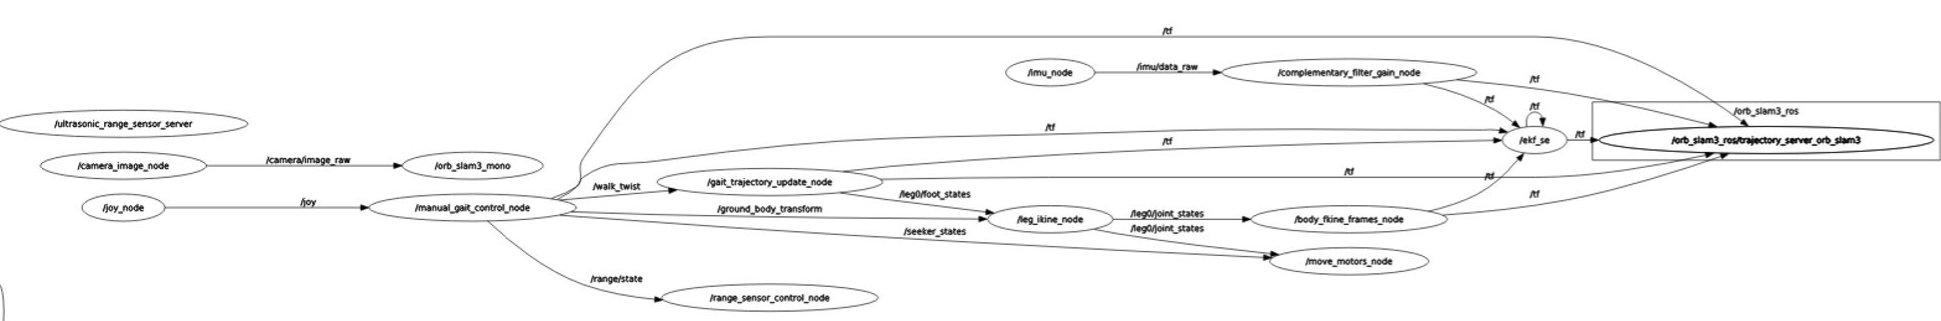
\includegraphics[scale=0.12]{figures/rosgraph.png}
    \caption{ Node design for ROS software architecture }
    \label{fig:rqt}
\end{figure}

In order to facilitation motion through the space we wish to map, a master controller node receives input from an Xbox controller to determine the desired body motion. This node outputs a twist vector and a body pose relative to the ground, as well as seeker gimble angles. The gait update node receives the twist vector and calculates new desired foot positions. An inverse kinematics node then calculates new joint angles, which are received by the motor driver node to actuate the servo motors.

\subsubsection{ Extended Kalman Filter (EKF)}

For continuous body pose estimation, the robot\_localization ROS package \cite{robotlocalization} was used to implement an extended Kalman filter (EKF). This filter receives the commanded twist vector in the ground frame, as well as IMU sensor data in the body frame, and estimates the robot's pose relative to the fixed odometry frame over time.
